
%==========================================================================================
\section{Ressourcenbeschränkte Projektplanung und Zusatzkapazitäten}

\begin{frame}[noframenumbering]
\frametitle{Gliederung}
\tableofcontents[current, hideallsubsections]
\end{frame}

\begin{frame}[t]
\frametitle{Ressourcenbeschränkte Projektplanung}
\begin{center}
\includegraphics[page=3, width=\textwidth]{images/rcpsp.pdf}\\
\end{center}

{\small
Projektdauerminimale Einplanung von Arbeitsgängen $j$ mit gegebenen
\begin{itemize}
\itemsep0em
\item Dauern $d_j$
\item Ressourcenbelastungen $k_{jr}$
\item Reihenfolgebeziehungen $i \in \mathcal{P}_j$
\item Kapazitätsrestriktionen $K_r$
\end{itemize}
}
\end{frame}

%==========================================================================================

\begin{frame}
\frametitle{Projektdauer und Deckungsbeitrag}
\begin{small}
Praxisbeispiel: Aufarbeitung eines Triebwerks durch Dienstleister
\begin{itemize}
\item Projektdauer {\large $\downarrow$} $\implies$ Zahlungsbereitschaft {\large $\uparrow$\\}
\item Überstunden {\large $\uparrow$} $\implies$ Projektdauer {\large $\downarrow$} Kosten {\large $\uparrow$}\\
\item[] \begin{tabbing}
$\Rightarrow$ \= Maximierung des Deckungsbeitrags als Trade-off zwischen\\
\>Dauer- und Kostenminimierung
\end{tabbing}

\end{itemize}
\end{small}
\begin{center}
\includegraphics[page=3,scale=0.29]{images/ErloesKostenDeckungsbeitrag.pdf}
\end{center}
\end{frame}

%==========================================================================================

\begin{frame}[t]
	\frametitle{Projektplanung mit Zusatzkapazitäten}
	\begin{center}
		\includegraphics[width=\textwidth]{images/RCPSPOCIntro.pdf}\\
	\end{center}
	
	{\small
		Deckungsbeitragsmaximale Einplanung von Arbeitsgängen mit zusätzlich gegebenen
		\begin{itemize}
			\itemsep0em
			\item Kostensätzen für Zusatzkapazität $\kappa_r$
			\item oberen Schranken für Zusatzkapazität $\overline{z}_r$
			\item projektdauerabhängigen Erlösen $u_t$
		\end{itemize}
	}
\end{frame}

%%%%%%%%%%%%%%%%%%%%%%%%%%%%%%%%%%%%%%%%%%%%%%%%%%%%%%%%%%%%%%%%%%%%%%%%%%%%%%%%%%%%%%%%%%%%%%%%%%%%%%%%%

\begin{frame}
	\frametitle{Entscheidungsmodell: RCPSP-OC}
	\begin{footnotesize}
		\begin{itemize}
			\item Zielfunktion\\[-7mm]
			\[
			\mbox{max } \sum_{t=EFT_{J+1}}^{LFT_{J+1}} u_t \cdot x_{{J+1},t} - \sum_{r \in \mathcal{R}} \sum_{t \in \mathcal{T}} \kappa_r \cdot z_{rt}
			\]
			
			\item Einmalige Durchführung
			\[
			\sum_{t=EFT_j}^{LFT_j} x_{jt} = 1 \,\,\,\quad\quad\quad\quad\quad\quad\quad\quad\quad\quad\quad j \in \mathcal{J}\textcolor{white}{, t \in \mathcal{T}}
			\]
			
			\item Reihenfolgerestriktionen
			\[
			\sum_{t=EFT_i}^{LFT_i} x_{it} \cdot t \leq \sum_{t=EFT_j}^{LFT_j} x_{jt} \cdot t - d_j \,\,\:\:\:\quad\quad\quad j \in \mathcal{J}, \; i \in \mathcal{P}_j
			\]
			
			\item Kapazitätsrestriktionen
			\[
			\sum_{j=1}^{J} \sum_{\tau=t}^{t+d_j-1} k_{jr} \cdot x_{j\tau} \leq K_r + z_{rt} \,\,\:\:\:\:\:\quad\quad\quad\quad r \in \mathcal{R}, \; t \in \mathcal{T}
			\]
			
			\item Obere Schranke für Zusatzkapazität\\[-3mm]
			\[
			z_{rt} \leq \overline{z}_r \,\;\;\quad\quad\quad\quad\quad\quad\quad\quad\quad\quad\quad\quad\quad\quad r \in \mathcal{R}, \; t \in \mathcal{T}
			\]
		\end{itemize}
	\end{footnotesize}
\end{frame}

%%%%%%%%%%%%%%%%%%%%%%%%%%%%%%%%%%%%%%%%%%%%%%%%%%%%%%%%%%%%%%%%%%%%%%%%%%%%%%%%%%%%%%%%%%%%%%%%%%%%%%%%%

\section{Heuristische Lösungsverfahren}

\begin{frame}[noframenumbering]
\frametitle{Gliederung}
\tableofcontents[current,currentsubsection]
\end{frame}

\begin{frame}
\frametitle{Genetische Algorithmen}
Repräsentationen im Überblick
\begin{itemize}
	\item \small{Startzeit zwischen Reihenfolge- und Ressourcenzulässigkeit}\\[2mm]
	\begin{small}
	\begin{tabular}{cp{7.5cm}}
	\hline
	Individuum & Planerzeugung\\
	\hline
	$(\lambda)$ & Vervollständigung jeder Alternative ohne ZK\\	
	$(\lambda|\tau)$& Startzeit beliebig in Zeitfenster\\
	$(\lambda|\beta)$& Startzeit an Zeitfensterrand\\
	\end{tabular}
	\end{small}\\[4mm]
	
	\item \small{Vorbestimmung des Ressourcenprofils}\\[2mm]
	\begin{small}
		\begin{tabular}{cp{7.5cm}}
			\hline
			Individuum & Planerzeugung\\
			\hline
			$(\lambda|z_{rt})$ & Kapazität entspricht $K_r+z_{rt}$\\
			$(\lambda|z_r)$ & Kapazität entspricht $K_r+z_{r}$\\
		\end{tabular}
	\end{small}
\end{itemize}
\end{frame}

%%%%%%%%%%%%%%%%%%%%%%%%%%%%%%%%%%%%%%%%%%%%%%%%%%%%%%%%%%%%%%%%%%%%%%%%%%%%%%%%%%%%%%%%%%%%%%%%%%%%%%%

\subsection{Feste Kapazität $(\lambda|z_{r})$}
\begin{frame}[noframenumbering]
	\frametitle{Gliederung}
	\tableofcontents[currentsubsection]
\end{frame}


\begin{frame}
	\frametitle{Planerzeugung $(\lambda|z_{r})$: Einplanung AG 2}
	\includegraphics<1>[page=1, scale=0.75]{images/SSGSzr.pdf}
	\includegraphics<2>[page=2, scale=0.75]{images/SSGSzr.pdf}
\end{frame}

\begin{frame}
	\frametitle{Genetischer Algorithmus $(\lambda|z_{r})$}
	\begin{small}
		\begin{center}
			\begin{tabular}{rl}
				\hline 
				Individuum & $(\lambda|z_{r})=(0,1,3,5,2,4,6,7|0,2,2,0,3,0,\ldots)$\parbox[c][40pt][c]{0pt}{}\tabularnewline
				\hline 
				Initialpopulation & $z_{r}=$ Zufallszahl aus $\{0, \ldots, \overline{z}_{r}\} \; \forall r$\tabularnewline
				\hline 
				Rekombination & One Point Crossover\tabularnewline
				\hline 
				Mutation & $z_{r}=$ Zufallszahl aus $\{0, \ldots, \overline{z}_{r}$\} mit $P_{mutate}$\tabularnewline
				\hline 
				Fitness & Deckungsbeitrag von kodiertem Plan\tabularnewline
				\hline
			\end{tabular}
		\end{center}
	\end{small}
\end{frame}

%%%%%%%%%%%%%%%%%%%%%%%%%%%%%%%%%%%%%%%%%%%%%%%%%%%%%%%%%%%%%%%%%%%%%%%%%%%%%%%%%%%%%%%%%%%%%%%%%%%%%%%

\subsection{Vervollständigung ohne ZK $(\lambda)$}
\begin{frame}[noframenumbering]
	\frametitle{Gliederung}
	\tableofcontents[currentsubsection]
\end{frame}

\begin{frame}[t]
	\frametitle{Planerzeugung $(\lambda)$: Einplanung AG 2}
	\begin{center}
		\includegraphics<1>[page=1, scale=0.73]{images/ssgsoc.pdf}
		\includegraphics<2>[page=2, scale=0.73]{images/ssgsoc.pdf}
		\includegraphics<3>[page=3, scale=0.73]{images/ssgsoc.pdf}
		\includegraphics<4>[page=4, scale=0.73]{images/ssgsoc.pdf}
		\includegraphics<5>[page=5, scale=0.73]{images/ssgsoc.pdf}
		\includegraphics<6>[page=6, scale=0.73]{images/ssgsoc.pdf}
		\includegraphics<7>[page=5, scale=0.73]{images/ssgsoc.pdf}\\
		
		\only<1>{
			Bisher Arbeitsgang 1 eingeplant.
			\textcolor{white}{$\mbox{DB} = u_8 - \sum_r \sum_t \kappa_r z_{rt} = 20\mbox{ GE} - 20\mbox{ GE} = 0\mbox{ GE}$}
		}
		
		\only<2>{
			Früheste Reihenfolgezulässigkeit $\underline{t}$\\
			\textcolor{white}{$\mbox{DB} = u_8 - \sum_r \sum_t \kappa_r z_{rt} = 20\mbox{ GE} - 20\mbox{ GE} = 0\mbox{ GE}$}
		}
		
		\only<3>{
			Früheste Reihenfolgezulässigkeit $\underline{t}$\\
			$\mbox{DB} = u_8 - \sum_r \sum_t \kappa_r z_{rt} = 20\mbox{ GE} - 20\mbox{ GE} = 0\mbox{ GE}$
		}
		
		\only<4>{
			Inkrementiere\\
			$\mbox{DB} = u_8 - \sum_r \sum_t \kappa_r z_{rt} = 20\mbox{ GE} - 20\mbox{ GE} = 0\mbox{ GE}$
		}
		
		\only<5>{
			Inkrementiere\\
			$\mbox{DB} = u_9 - \sum_r \sum_t \kappa_r z_{rt} = 15\mbox{ GE} - 10\mbox{ GE} = 5\mbox{ GE}$
		}
		
		\only<6>{
			Früheste Ressourcenzulässigkeit $\overline{t}$\\
			$\mbox{DB} = u_10 - \sum_r \sum_t \kappa_r z_{rt} = 0\mbox{ GE} - 0\mbox{ GE} = 0\mbox{ GE}$
		}
		
		\only<7>{
			Bester Kandidat für Einplanungszeitpunkt\\
			$\mbox{DB} = u_9 - \sum_r \sum_t \kappa_r z_{rt} = 15\mbox{ GE} - 10\mbox{ GE} = 5\mbox{ GE}$
		}
	\end{center}
\end{frame}

\begin{frame}
	\frametitle{Genetischer Algorithmus $(\lambda)$}
	\begin{small}
		\begin{center}
			\begin{tabular}{rl}
				\hline 
				Individuum & $(\lambda)=(0,1,4,2,5,3,6,7)$\parbox[c][40pt][c]{0pt}{}\tabularnewline
				\hline 
				Initialpopulation & Regret-Based Biased Random Sampling (LFTs)\tabularnewline
				\hline 
				Rekombination & One Point Crossover\tabularnewline
				\hline 
				Mutation & Neighborhood Swap\tabularnewline
				\hline 
				Fitness & Deckungsbeitrag von kodiertem Plan\tabularnewline
				\hline 
			\end{tabular}
		\end{center}
	\end{small}
\end{frame}

%%%%%%%%%%%%%%%%%%%%%%%%%%%%%%%%%%%%%%%%%%%%%%%%%%%%%%%%%%%%%%%%%%%%%%%%%%%%%%%%%%%%%%%%%%%%%%%%%%%%%%%

\subsection{Wahl in Zeitfenster $(\lambda|\tau)$}
\begin{frame}[noframenumbering]
	\frametitle{Gliederung}
	\tableofcontents[currentsubsection]
\end{frame}

\begin{frame}[t]
	\frametitle{Planerzeugung $(\lambda|\tau)$: Einplanung AG 2}
	\includegraphics<1-2>[page=1, scale=0.7]{images/ssgstau.pdf}
	\includegraphics<3>[page=2, scale=0.7]{images/ssgstau.pdf}
	\only<1>{\[ ST_2 = \overline{t} - [ (\overline{t}-\underline{t}) \cdot \tau ] \]}
	\only<2>{\[ ST_2 = 4 - [ (4-1) \cdot 0{,}3 ] = 4 - [ 0{,}9 ] = 3\]}
	\only<3>{\[ ST_2 = 4 - [ (4-1) \cdot 0{,}9 ] = 4 - [ 2{,}7 ] = 1\]}
\end{frame}

\begin{frame}
	\frametitle{Genetischer Algorithmus $(\lambda|\tau)$}
	\begin{small}
		\begin{center}
			\begin{tabular}{rl}
				\hline 
				Individuum & $\begin{pmatrix}\lambda\\\tau\end{pmatrix}=\begin{pmatrix}0,1,3,5,2,4,6,7\\0,0.3,0.5,0.8,0.9,0.2,0.1,0.2\end{pmatrix}$\parbox[c][40pt][c]{0pt}{}\tabularnewline
				\hline 
				Initialpopulation & $\tau_j=$ Zufallszahl aus $[0, 1) \; \forall j$\tabularnewline
				\hline 
				Rekombination & Gemeinsamer OPC mit $\lambda$\tabularnewline
				\hline 
				Mutation & $\tau_j=$ Zufallszahl aus $[0,1)$ mit $P_{mutate}$\tabularnewline
				\hline 
				Fitness & Deckungsbeitrag von kodiertem Plan\tabularnewline
				\hline 
			\end{tabular}
		\end{center}
	\end{small}
\end{frame}

%%%%%%%%%%%%%%%%%%%%%%%%%%%%%%%%%%%%%%%%%%%%%%%%%%%%%%%%%%%%%%%%%%%%%%%%%%%%%%%%%%%%%%%%%%%%%%%%%%%%%%%

\subsection{Zeitfenstergrenzen $(\lambda|\beta)$}
\begin{frame}[noframenumbering]
	\frametitle{Gliederung}
	\tableofcontents[currentsubsection]
\end{frame}

\begin{frame}
	\frametitle{Planerzeugung $(\lambda|\beta)$: \only<1-2>{untere}\only<3-6>{obere} Einplanung}
	
	\includegraphics<1>[page=1, scale=0.75]{images/SSGSbetaLower.pdf}
	\includegraphics<2>[page=2, scale=0.75]{images/SSGSbetaLower.pdf}
		
	\includegraphics<3>[page=1, scale=0.75]{images/SSGSbetaUpper.pdf}
	\includegraphics<4>[page=2, scale=0.75]{images/SSGSbetaUpper.pdf}
	\includegraphics<5>[page=3, scale=0.75]{images/SSGSbetaUpper.pdf}
	\includegraphics<6>[page=4, scale=0.75]{images/SSGSbetaUpper.pdf}
\end{frame}

\begin{frame}
	\frametitle{$(\lambda|\beta)$-Varianten}
	\begin{itemize}
		\item Arbeitsgangzuordnung: AG $j=\lambda_i$ nutzt ZK, gdw.
		\begin{itemize}
			\item $\beta_i=1$ (Listenposition assoziiert)
			\item $\beta_j=1$ (AG-Nummer assoziiert)\\[4mm]
		\end{itemize}
		\item Einplanungsart
		\begin{itemize}
			\item "`von unten"': Nutze erst Normalkapazität
			\item "`von oben"': Nutze erst Überstunden\\[4mm]
		\end{itemize}
		\item Crossover
		\begin{itemize}
			\item Gemeinsamer One Point Crossover
			\item Zwei getrennte One Point Crossovers\\[5mm]
		\end{itemize}
		\item[$\implies$] Insgesamt $2 \cdot 2 \cdot 2 = 8$ unterschiedliche Varianten
	\end{itemize}
\end{frame}

\begin{frame}
	\frametitle{Genetischer Algorithmus $(\lambda|\beta)$}
	\begin{small}
		\begin{center}
			\begin{tabular}{rl}
				\hline 
				Individuum & $\begin{pmatrix}\lambda\\\beta\end{pmatrix}=\begin{pmatrix}0,1,3,5,2,4,6,7\\0,1,1,0,1,0,1,0\end{pmatrix}$\parbox[c][40pt][c]{0pt}{}\tabularnewline
				\hline 
				Initialpopulation & $\beta_i=$ Zufallszahl aus $\{0,1\} \; \forall i \in \mathcal{J}$\tabularnewline
				\hline 
				Rekombination & One Point Crossover\tabularnewline
				\hline 
				Mutation & $\beta_i=\neg \beta_i$ mit $P_{mutate}$\tabularnewline
				\hline 
				Fitness & Deckungsbeitrag von kodiertem Plan\tabularnewline
				\hline 
			\end{tabular}
		\end{center}
	\end{small}
\end{frame}

%%%%%%%%%%%%%%%%%%%%%%%%%%%%%%%%%%%%%%%%%%%%%%%%%%%%%%%%%%%%%%%%%%%%%%%%%%%%%%%%%%%%%%%%%%%%%%%%%%%%%%%

\section{Numerische Ergebnisse}
\begin{frame}[noframenumbering]
\frametitle{Gliederung}
\tableofcontents[current, hidesubsections]
\end{frame}


\begin{frame}[t]
\frametitle{Numerische Ergebnisse}
\begin{footnotesize}
\textbf{Parameter:} Populationsgröße $=80$, $P_{mutate}=5\%$\\

\begin{center}
	\begin{tabular}{ccc}
		\multicolumn{3}{c}{\textbf{Testinstanzen}}\\
		Datensatz & \#Projekte & Zeitlimit\\
		j30 & 199 & $1s$\\
		j120 & 586 & $15s$
	\end{tabular}
\end{center}

\begin{center}	
\tabcolsep=0.16cm
\begin{tabular}{|c|rc|rc|}
	\hline
	\rule{0pt}{4mm} & \multicolumn{2}{c|}{j30} & \multicolumn{2}{c|}{j120}\\[1mm]
	 & $\varnothing$ Gap & $\varnothing$ Rang & $\varnothing$ Gap & $\varnothing$ Rang \\[3pt]
	\hline
   $(\lambda|z_{rt})$ & 1.41\% & 1.98 & 1.91\% & 3.63\\
	\hline
   $(\lambda|z_r)$ & 3.01\% & 2.60 & \textbf{0.95\%} & \textbf{2.19}\\
	\hline
	$(\lambda|\beta)$ & 2.80\% & 2.37 & 1.61\% & 2.97\\
	best & & & & \\
	\hline
	$(\lambda|\beta)$&5.27\% & 4.39 & 11.76\% & 9.56\\
	worst & & & & \\
	\hline
	$(\lambda|\tau)$&2.45\% & 2.98 & 4.48\% & 6.08\\
	\hline
	$(\lambda)$& \textbf{1.20\%} &\textbf{1.78} & 5.04\% & 5.40\\
	\hline
\end{tabular}
\end{center}

Erlösfunktion setzt minimal erreichbaren Deckungsbeitrag auf 0 $\implies$ Rationalskaliert

\end{footnotesize}	

\end{frame}

\section{Ausblick}

\begin{frame}[noframenumbering]
\frametitle{Gliederung}
\tableofcontents[current, hidesubsections]
\end{frame}

\begin{frame}
\frametitle{Ausblick}
\begin{itemize}
\item Verbesserung der Genetischen Algorithmen
	\begin{itemize}
	\item Stellschrauben: $P_{mutate}$, Populationsgröße, Zeitlimits
	\item Anpassung von Mutation und Crossover\\[6mm]
	\end{itemize}
\item Techniken führender RCPSP-Heuristiken
	\begin{itemize}
	\item Vorwärts-Rückwärts-Verbesserung
	\item Fitnessbasierte Paarbildung und Crossover
	\item Zweite Suchphase in Nachbarschaft\\[6mm]
	\end{itemize}
\item Problemspezifischer B\&B-Algorithmus
\end{itemize}
\end{frame}




